\documentclass[11pt,letterpaper]{article}
\usepackage[T1]{fontenc}
\usepackage[utf8]{inputenc}
\usepackage{lmodern,microtype}
\usepackage[margin=0.94in,headheight=15pt]{geometry}
\usepackage{amsmath,amssymb,amsthm,mathtools,stmaryrd}
\usepackage{booktabs,tabularx,longtable,array}
\usepackage{xcolor,listings,enumitem,needspace,fancyhdr,titlesec,etoolbox}
\usepackage[most]{tcolorbox}
\usepackage{tikz}
\usetikzlibrary{arrows.meta,positioning}
\usepackage{xurl}
\usepackage[colorlinks=true,linkcolor=ink,citecolor=ink,urlcolor=accent]{hyperref}
\usepackage{bookmark}
\definecolor{ink}{HTML}{18384D}
\definecolor{accent}{HTML}{226E79}
\definecolor{pale}{HTML}{F2F6F7}
\definecolor{linegray}{HTML}{CCD8DC}
\titleformat{\section}{\Large\sffamily\bfseries\color{ink}}{\thesection}{.6em}{}
\titleformat{\subsection}{\large\sffamily\bfseries\color{ink}}{\thesubsection}{.6em}{}
\titleformat{\subsubsection}{\normalsize\bfseries}{\thesubsubsection}{.6em}{}
\titlespacing*{\section}{0pt}{2.5ex plus 1ex}{1.0ex}
\titlespacing*{\subsection}{0pt}{2ex plus .7ex}{.7ex}
\setlength{\parindent}{0pt}
\setlength{\parskip}{.4em}
\setlength{\emergencystretch}{2em}
\setcounter{tocdepth}{1}
\setlist{nosep,leftmargin=1.5em}
\renewcommand{\arraystretch}{1.15}
\newcolumntype{Y}{>{\raggedright\arraybackslash}X}
\newcolumntype{P}[1]{>{\raggedright\arraybackslash}p{#1}}
\newcommand{\code}[1]{\nolinkurl{#1}}
\newcommand{\Facet}{\textsc{Facet}}
\newcommand{\N}{\mathbb N}
\newcommand{\Z}{\mathbb Z}
\newcommand{\Q}{\mathbb Q}
\newcommand{\R}{\mathbb R}
\newcommand{\E}{\mathcal E}
\newcommand{\FV}{\operatorname{FV}}
\newcommand{\Valid}{\operatorname{Valid}}
\newcommand{\Rep}{\operatorname{Rep}}
\newcommand{\Spec}{\operatorname{Spec}}
\newcommand{\den}[1]{\llbracket #1\rrbracket}
\newcommand{\coeff}[2]{[#1]#2}
\newcommand{\src}[2]{\href{#1}{#2}}
\newtcolorbox{claimbox}[1][]{colback=pale,colframe=linegray,boxrule=.5pt,arc=1mm,left=9pt,right=9pt,top=7pt,bottom=7pt,breakable,#1}
\lstset{basicstyle=\small\ttfamily,columns=fullflexible,keepspaces=true,
 breaklines=true,showstringspaces=false,frame=single,rulecolor=\color{linegray},
 backgroundcolor=\color{pale},framesep=6pt,xleftmargin=6pt,xrightmargin=6pt,
 aboveskip=.7em,belowskip=.7em,tabsize=2}
\newtheorem{proposition}{Proposition}[section]
\newtheorem{definition}[proposition]{Definition}
\newtheorem{example}[proposition]{Example}
\numberwithin{equation}{section}
\pagestyle{fancy}
\fancyhf{}
\fancyhead[L]{\small\sffamily Facet / A proof--CAS language}
\fancyhead[R]{\small\sffamily Second-round proposal}
\fancyfoot[C]{\small\thepage}
\renewcommand{\headrulewidth}{.3pt}
\hypersetup{pdftitle={Facet: Mathematical Objects with Certified Computational Presentations},pdfauthor={OpenAI, prepared for Vladimir Reshetnikov},pdfsubject={Second-round proof-language design; Lean, Leant, verified computer algebra}}

\pretocmd{\section}{\Needspace{8\baselineskip}}{}{}
\pretocmd{\subsection}{\Needspace{5\baselineskip}}{}{}
\begin{document}
\begin{titlepage}
\color{ink}
{\sffamily\large PROOF-LANGUAGE DESIGN / SECOND ITERATION\par}
\vspace*{1.0in}
{\sffamily\bfseries\fontsize{39}{44}\selectfont Facet\par}
\vspace{.24in}
{\sffamily\bfseries\fontsize{25}{31}\selectfont Mathematical Objects with\\Certified Computational\\Presentations\par}
\vspace{.3in}
{\sffamily\Large A Lean-hosted language joining mathematical\newline arguments, symbolic computation, and checked evidence\par}
\vspace{.45in}
\begin{claimbox}
\color{black}
\textbf{The proposal.} Make the mathematical object stable, make its computational
presentations explicit and reusable, and make every transformation return its
precise relation to that object. A calculation is then a proof step with an
executable implementation, not an answer imported from another semantic world.
\end{claimbox}
\vfill
\rule{\textwidth}{.7pt}
Prepared for Vladimir Reshetnikov\par
OpenAI\par
5 September 2026, Pacific time\par
\vspace{.15in}
{\small\color{black}Status: research proposal and static source review. The language,
protocol, and interfaces described here are specifications, not a delivered
implementation. Mathematical derivations are supplied; no new Lean program or
compiler was built, and no usability or performance improvement was measured.}
\end{titlepage}

\begin{abstract}
\noindent The first brainstorming round converged on a sensible architecture:
Lean checking, claim-centered documents, scoped obligations, fixed meanings,
replayable evidence, and fair comparisons against equally equipped Lean. Repeating
that architecture with new keywords would contribute little. This proposal instead
makes \emph{certified computational presentations of mathematical objects} the
organizing abstraction. A polynomial can have a theorem-friendly definition and
an efficient coefficient representation; a formal series can have a finite-jet
presentation without being confused with an analytic function; a real algebraic
number can have an isolating interval without becoming an approximate number.
The same language can define these objects, calculate with them using verified
algorithms, and incorporate the resulting exact, conditional, or approximate
facts into a mathematical argument.

The difficult boundaries are specified rather than delegated to an unspecified
CAS: representation transport has direction and guards; finite observations are
not full equality; branch choices are retained; algorithm correctness is distinct
from trustworthy execution; and complete search failure is not automatically a
proof of negation. Worked designs cover binomial inversion, local differentiation,
polynomial recurrences for autonomous equations, Abel generating functions,
rational-function cancellation, and radical denesting. A typed Leant adapter,
a publication format, a staged implementation plan, an adversarial suite, and
responses to all twenty-two next-round questions in the two synthesis reports
complete the proposal. The proposed contribution is an integration and a set of
concrete contracts, not a claim to have invented certified computer algebra.
\end{abstract}

\section*{The design decision}
\addcontentsline{toc}{section}{The design decision}
\begin{claimbox}
\textbf{Build a mathematical workspace, not an English wrapper around tactics.}
The first implementation should be a Lean package with two authoring surfaces:
ordinary Lean and a small mathematical-step dialect. Both share object interfaces,
certified computations, obligation tracking, and publication evidence. New syntax
is optional; exact semantic contracts are not.
\end{claimbox}

The distinctive move is to promote the \emph{definition--representation--algorithm}
interface to the same status as the proof interface. It is usually not enough to
say ``do the algebra'' more tersely. The system must know \emph{which algebra},
\emph{which object it represents}, and \emph{what a successful calculation licenses}
in the original argument. A proof assistant with this interface becomes a useful
CAS without delegating mathematical meaning to an external program.

The initial investment should be narrow: exact polynomial computation and a
finite-sum view, followed by local calculus and formal-series coefficients. General
symbolic integration, unrestricted natural-language interpretation, automatic
representation discovery, and a new kernel are not prerequisites. If the new
surface adds no value beyond the shared library and document view, the library
and view are the successful result of the project.

\clearpage
\begingroup
\setlength{\parskip}{0pt}
\small
\tableofcontents
\endgroup
\clearpage

\section{What this second round should change}\label{sec:round}
\subsection{What is inherited, and from which evidence}
I read the two requested synthesis reports at Brainstorm revision
\code{494be9d5ab41a5ae219fc6f800e6aee3c93bce39}: \emph{Mathematical Ideas, Checked
Evidence} and \emph{Nine Blueprints for a Mathematician's Proof Language over Lean}
\cite{synthesis,blueprints}. The first supplies a carefully qualified common
protocol, mathematical stress tests, a detailed Leant review, and ten questions.
The second adds a corpus-level lexical audit, an annotated-theorem proposal,
stronger emphasis on definition interfaces, and twelve additional questions.
Both incorporate corrections arising from comparison with the other. Their
agreement is useful design evidence, not independent experimental validation.

I retain their main commitments: existing Lean foundations, visible mathematical
claims, dependent scopes, an approved statement boundary, separate proof and
object synthesis, positive checking at the original goal, source-linked evidence,
and a comparison with Lean using the same helpers. I also retain the important
qualification that ordinary Lean already provides much of the necessary machinery.
For example, a polynomial identity should normally reuse existing proof-producing
algebraic normalization rather than motivate a second ring tactic
\cite{ring,synthesis,blueprints}.

\subsection{The additional commitments}

\begin{tabularx}{\textwidth}{@{}P{.27\textwidth}Y@{}}
\toprule
Inherited direction & More specific commitment in this proposal\\
\midrule
Certified views & A presentation is a typed relation to a fixed object, with
operation-specific preservation or reflection. Routes compose with dependent
guards; no universal equivalence flag is used.\\
Definitions matter & Definition packages publish stable laws, explicit
construction choices, executable representations, and proved bridges together.\\
Proof-producing automation & A computational operation has a verified algorithm
or a verified checker, and a separately specified execution path.\\
Scoped obligations & Conditional calculation results are dependent functions
of their missing premises, not temporary unconditional facts.\\
Honest synthesis outcomes & Mathematical negation, a counterexample, and
non-derivability in a searched calculus are different types of evidence.\\
Two frontends & Compare the surface, definition packages, and verified-CAS
services as separate interventions, not one indivisible product.\\
\bottomrule
\end{tabularx}


This is not a claim that none of the original proposals anticipated these ideas.
The first synthesis explicitly discusses directed views and observation-relative
replacement; the second emphasizes definition packages and theorem annotations.
The contribution here is to choose a concrete joint design and push its
computational consequences far enough to expose implementation obligations.

\subsection{Two corrections to overly optimistic interpretations}
First, a classification of source lines is not a measurement of removable work.
The secondary report records 90,637 tactic-like entries and classifies 32.3\% in
families it calls reconstructible. These are the report's lexical counts, not
measurements performed for this article. They neither establish a compression
factor nor show that the premises can be recovered without author input. The
reports themselves substantially qualify this interpretation after their mutual
review \cite{synthesis,blueprints}.

Second, replacing an adequacy flag by a list of abstracted nodes does not turn
metadata into a proof of adequacy. Even a correctly implemented, complete search
for derivations answers a question about \emph{derivability in its calculus}.
Without a further theorem connecting that question to the requested mathematical
proposition, exhaustion does not yield its negation. Section~\ref{sec:negative}
gives a precise counterexample and a provider interface that retains the useful
Leant distinctions without overstating their authority.

\subsection{Scope of the source review}
The code examples below were read at explicit commits, not inferred from report
snippets. ProveIt is inspected at \code{7c4e3f10}, the revision used by both
syntheses, and Leant at its retrieved public \code{main} revision
\code{3a40904b}. Full identities and file paths are in Appendix~\ref{app:sources}.
This is a targeted review, not a current whole-repository audit or a rebuild.
In particular, the syntheses' Leant working trees include uncommitted material;
those working trees are not identified with the public commit here.

\section{Three source examples and the actual source of verbosity}\label{sec:source}
\subsection{Binomial inversion: preserve the additive-group theorem}
The inspected \code{BinomialInversion.lean} separates an integer kernel identity
from its action on sequences. Its module-valued theorem assumes only
\code{[AddCommGroup M]}; integer coefficients act by scalar multiplication.
Ring-valued statements are additional specializations, not the foundation of the
result. The file already reuses a lower-triangular transform calculus
\cite{p-binomial}.

Its longer orthogonality proof handles an empty interval, introduces
$n=j+m$, converts an inclusive interval into a range, applies
\code{Nat.choose_mul}, moves natural coefficients to integers, and normalizes
products. These are not all the same task. Choosing $k=j+i$ is the mathematical
reindexing. Proving its coverage is necessary evidence. Repeatedly moving a
coefficient cast across a product is a reusable representation operation.

The right CAS interface is consequently \emph{integer kernel algebra followed
by the existing module-action theorem}. It must not reinterpret $M$ as a field
because a symbolic engine prefers field expressions. That would prove a less
general theorem, not the original theorem more naturally.

\subsection{Autonomous derivatives: locality is an input, not formatting}
The source theorem \code{AutonomousODE.iteratedDeriv_eq_comp} assumes an open set
$s$, the differential equation for $W$ on $s$, and derivative information about
$G_n$ only at the points $W(x)$ reached from $s$. It builds an eventual equality
near $x$ from the induction hypothesis on the open set, then applies derivative
congruence and the chain rule \cite{p-ode}.

The crucial source fragment is short enough to show directly:
\par\noindent\begin{minipage}{\linewidth}
\begin{lstlisting}
have heq : iteratedDeriv n W =f[nhds x] G n o W :=
  eventuallyEq_of_mem (hs.mem_nhds hx) (fun y hy => ih y hy)
rw [heq.deriv_eq]
\end{lstlisting}
\end{minipage}\par

This is an ASCII transcription of the mathematical shape, not compilable Lean.
The first line is not dispensable mathematics. It explains why an equality can
be differentiated. A language should package the open-set-to-neighborhood bridge
once, but should still expose the locality of the identity in its normal reading
view. It should also preserve range-local hypotheses rather than silently demand
that every $G_n$ be differentiable everywhere.

This file is already a good abstraction. A new frontend earns its place only if
it makes instances of the abstraction easier to construct, diagnose, or read.

\subsection{Abel series: an object law is more general than a constructor}
\code{AbelPolynomialSeries.lean} defines Abel polynomials over every commutative
ring, then works with formal power series over a commutative $\Q$-algebra. It
constructs a canonical series but proves the coefficient formula for
\emph{any} series $T$ satisfying $T=t\exp(-aT)$. It explicitly obtains substitution
admissibility, transports rational inverses through \code{algebraMap}, and handles
the constant coefficient separately \cite{p-abel}.

This example makes the definition interface central. A user says ``let $T$ satisfy
this equation''; the system must not replace that quantified $T$ by its favorite
constructor. Conversely, when a user asks to compute $T$ to finite order, an
executable representative is useful, provided it comes with a theorem connecting
it to the arbitrary $T$ under its stated law. The same interface should support
both activities without conflating them.

\begin{claimbox}
\textbf{Diagnosis.} The recurring obstruction is not simply the number of tactics.
It is the repeated reconstruction of a bridge between a mathematical law and the
representation in which an operation is convenient. \Facet{} makes that bridge
a reusable, checked part of the object's interface.
\end{claimbox}

\section{A language of mathematical actions}\label{sec:surface}
\subsection{A small stored language, not an unrestricted prose parser}
The stored document uses Lean expressions initially. New syntax organizes scopes,
objects, claims, calculations, and reasons. Natural-language input may propose an
edit, but it is not the authoritative stored meaning. Here and throughout,
\Facet{} blocks are \emph{proposed syntax}; they have not been compiled.

\par\noindent\begin{minipage}{\linewidth}
\begin{lstlisting}
within x : Real, hx : x != 1:
  calculate (x^2 - 1) / (x - 1)
    as x + 1
    by rational_expression_normalize
    using hx
\end{lstlisting}
\end{minipage}\par


The author supplies the relation being asserted and the meaningful premises.
The system selects an applicable representation, produces the polynomial
identity and denominator obligations, proves them, and records the bridge back
to the original real expression. The expanded view shows that route. Omitting
\code{hx} leaves a conditional result; it does not invent an assumption.

There are three principal actions. A \code{claim} requests a proof of an already
resolved proposition. A \code{calculate} requests a result under a specified
relation to a fixed input. An \code{object} declaration introduces either a
specified arbitrary object or an explicitly chosen construction. These actions
share one checking and dependency protocol.

\Needspace{16\baselineskip}
\subsection{Directions of reasoning should remain distinct}
\par\noindent\begin{minipage}{\linewidth}
\begin{lstlisting}
claim C from A, B by theorem application
reduce C to D by equivalence
suffices D for C by implication
obtain witness w, property hw from existence_theorem
choose r satisfying positive_root_spec(a) by algebraic_root
\end{lstlisting}
\end{minipage}\par


A reduction by equivalence owes both directions; a sufficiency step needs only
the direction $D\to C$. Existential elimination with \code{obtain} introduces a
witness in a controlled proof scope. A computational \code{choose} creates an
object with an explicit specification and commits that choice for later use.
These are different operations even when a conventional prose proof calls both
``choose.'' Classical choice remains available as a named noncomputable
construction under the project's axiom policy, not as an invisible CAS fallback.

\subsection{Mathematical decisions versus inferred consequences}
Routine inference may fill evidence for a fixed bound, apply a declared
homomorphism, or compose supplied implications. It may not choose a root branch,
change the coefficient structure, reorder quantifiers, replace an arbitrary
solution, or enlarge a theorem's hypotheses merely to make search succeed.
A stronger induction motive is a proposed plan edit, not a silent new induction
hypothesis. An explicitly requested \code{by auto} may search for another proof;
a named \code{by reindex} must use the reindexing contract it advertises.

The stored form of a successful step records stable identities for facts and
objects. The printer can say ``by the preceding identity,'' but insertion of a
new identity does not retarget the stored reference. Retargeting is an edit with
a semantic difference display. This adopts the stable-reference direction of
the first synthesis \cite{synthesis}.

\subsection{One argument can include calculation without becoming a trace}
The reader sees the selected map, the recurrence, the branch, and the key
hypotheses. Coefficient-vector multiplication and cast normalization normally
appear only on expansion. The reason to collapse an operation is that its
contract is understood and reused, not that a solver found its proof quickly.
A domination hypothesis can be central even when automation proves it; a long
integer normalization can be secondary even when it costs seconds to check.

This aims at mathematical communication, not a claim to reproduce the author's
private mental process. The criterion is whether a reader can recover the
argument and identify an invalid nearby step.

\section{The semantic core: stable objects, explicit presentations}\label{sec:present}
\subsection{An object is not its current printed or executable form}
An object declaration introduces a resolved Lean term or a variable with a
specification. Its identity includes its type, universe parameters, local
structures, and dependencies. A computational presentation is additional evidence
about that object; it is not permission to redefine it.

For example, $p\in R[X]$ may be displayed in factored form, computed as a sparse
coefficient map, and evaluated as a function. These are three useful interfaces,
but their equality tests have different strengths. Equality of polynomials
implies equality of their evaluation functions. The converse is false over a
finite field: $X^2-X$ induces the zero function over $\mathbf F_2$ but is not the
zero polynomial. A workspace must not collapse these objects because their
current samples agree.

\begin{definition}[Exact computational presentation]
For a mathematical type $A$ in a fixed context, an exact presentation package
contains a data type $D$, a validity predicate $\Valid:D\to\mathrm{Prop}$, and an
interpretation
\[
 \operatorname{decode}:\{d:D\mid\Valid(d)\}\longrightarrow A.
\]
A presentation of $a:A$ consists of valid data $d$ and a proof
$\operatorname{decode}(d)=a$. No inverse map $A\to D$ is required.
\end{definition}

The lack of a universal encoder is intentional. An arbitrary real function may
have no available finite computational description. It can still participate as
an opaque mathematical object through its laws. A procedure may return
\code{Unsupported} when no applicable presentation is available without making a
claim about the object itself.

Validity includes such conditions as sparse-map invariants, dimensions,
coefficient domains, nonzero denominators, or unique-root isolation. These are
proved invariants of data, not trusted tags attached by a producer. Dependent
indices remain in the package: a representation of an $m\times n$ matrix must
not lose its dimensions when it crosses a service boundary.

\subsection{Observational presentations deliberately carry less information}
Some useful representations are not exact encodings of the entire object.
An interval encloses a real number; a finite jet records some coefficients of a
series; a finite table samples a function. Such a package uses a relation
\[
 V:D\to A\to\mathrm{Prop}
\]
with the meaning stated explicitly. It is not given the functionality property
of an exact presentation unless that property has actually been proved.


\begin{tabularx}{\textwidth}{@{}P{.22\textwidth}YP{.28\textwidth}@{}}
\toprule
Presentation & Certified relation & What it does not imply\\
\midrule
Sparse polynomial & $\operatorname{decode}(d)=p$ & That an arbitrary function
has this polynomial representation.\\
Jet through degree $N$ & $\forall k\le N,\ d_k=[X^k]F$ & Equality of two full
series with equal jets.\\
Rational interval & $\ell\le x\le u$ & $x=(\ell+u)/2$ or equality of enclosed
objects.\\
Algebraic root descriptor & $p(x)=0$, $\ell<x<u$, and uniqueness in the interval
& Minimality of $p$, unless separately certified.\\
Local function identity & $f=^{\mathcal N(x)}g$ & Global equality of $f$ and $g$.\\
Solution-set presentation & $P(x)\leftrightarrow Q(x)$ on a specified domain &
A preferred witness or a branch selection.\\
\bottomrule
\end{tabularx}


This classification is the main defense against CAS answers that look right but
prove too much. It also gives the user an informative result when exact equality
is unavailable: a proved enclosure or a finite-order identity is useful without
being mislabeled as an exact symbolic answer.

\subsection{An operation exports a theorem, not an untyped expression}
A simple exact operation has a mathematical specification $f:A\to B$, an
algorithm $F:D\to E$, and a theorem saying that valid presentations of $a$ are
sent to valid presentations of $f(a)$. A more general operation advertises a
relation $R(a,b)$ rather than equality to a named function. Examples include an
upper bound, a factorization, a selected root, and a sufficient condition.

The public result of an operation is therefore a dependent pair
\[
 (b,\pi):\sum_{b:B}R(a,b),
\]
possibly under explicit prerequisites. A request for \emph{all} roots has a
coverage specification; a request for \emph{a} root has only an existence-and-
selection specification. Returning several roots does not meet the all-roots
contract without coverage evidence.

Not every calculation has a canonical output. Factor order, root enumeration,
bases of kernels, and polynomial normal forms can vary. The chosen data object
is retained; later proof-only changes may replace its evidence but not silently
select a new witness. Representation changes that decode to the same retained
object can be automatic within a declared policy.

\subsection{Capabilities, not one universal algebra domain}
Each operation names its required algebraic interface. Integer-linear kernel
operations need an additive commutative group for their action. Commutative
polynomial normalization requires the corresponding ring laws. A multiplicative
inverse in a general ring needs a unit witness. Field division and order
comparisons need different capabilities. These requirements are part of the
instantiated theorem, not merely the engine's preferred runtime type.

An identity proved universally in $\Z[X_1,\ldots,X_r]$ can be transported to any
commutative ring by evaluation. An identity involving rational constants can be
transported into a commutative $\Q$-algebra using its algebra map. Neither transport
requires reflection of equality along the map. Reflection is a separate theorem
needed when the argument tries to infer an equality in the source from an equality
in the target. This difference is particularly important for specialization and
quotient rings.

\section{A calculus for guarded transformations}\label{sec:contracts}
\subsection{Why the underlying theorem should remain ordinary Lean}
The two syntheses make a strong case for defining most methods as ordinary
theorems with role annotations \cite{synthesis,blueprints}. \Facet{} adopts that
approach. The theorem type is the logical contract. A policy record says which
arguments the author selects, which premises a routine profile may attempt,
which relation is displayed, and what computational implementation is available.
A normalizer is connected by its correctness theorem; it is not forced into the
same implementation shape as a single theorem application.

Roles are attached to a project-owned interface with named, type-checked fields.
The interface is explicitly implemented by an application of the underlying
library theorem. This extra stable wrapper is preferable to treating an upstream
binder name as a permanent identifier. Reordering or renaming library binders
then breaks one implementation rather than silently changing the meaning of a
role in many documents. The wrapper and its maintenance cost must be included
in evaluation.

Logical interface, algorithm, routine profile, and presentation template have
separate versions. Their hashes identify what was used; they do not prove its
correctness. The instantiation of the theorem remains the logical authority.

\subsection{A conditional result is a function of its premises}
Suppose cancellation produces the desired result only under $g:x\ne1$. The
stored result may contain the term $x+1$ immediately, but its evidence is
\[
 \pi:(x\ne1)\to \frac{x^2-1}{x-1}=x+1.
\]
Until $g$ is supplied, the workspace does not add the displayed equality as an
unconditional local fact. It adds a \emph{conditional calculation}, visibly
marked with its exact missing premise.

The general form is a telescope, not a bag of conditions:
\[
 K:\Pi(h_1:G_1)\,\Pi(h_2:G_2(h_1))\cdots
       \Pi(h_r:G_r(h_1,\ldots,h_{r-1})).\ \sum_{b:B}R(a,b).
\]
A constructed object may itself depend on these premises or on witnesses they
introduce. The system must not exchange $\Pi h\,\Sigma b$ with
$\Sigma b\,\Pi h$ just because both print as ``a result under assumptions.''
These interfaces retain precisely the dependencies that a remote producer must
not guess from an unordered list of hypothesis strings.

The ledger tracks ordinary Lean obligations and their scope. Roles such as
\emph{domain}, \emph{branch}, \emph{coverage}, \emph{locality}, and \emph{computation}
are useful for explanation and provider selection; they do not change the logic
or make a difficult proposition routine.

\subsection{Composition has a direction and a proof}
Let $V(a,b)$ and $W(b,c)$ be certified relations. Their relational composition is
\[
 (V;W)(a,c)\;\Longleftrightarrow\;
 \exists b,\ V(a,b)\land W(b,c).
\]
To display the result as a desired relation $R(a,c)$, the package must provide
\[
 \forall a,b,c,\quad V(a,b)\to W(b,c)\to R(a,c).
\]
There is no general rule that calls this result equality. Equality-to-enclosure
composition gives an enclosure; implication followed by implication gives an
implication; a many-to-one map generally provides preservation but not reflection.

A route certificate records the chosen intermediate object, each instantiated
bridge, the guard proofs in dependency order, and the final relation. It can be
checked without re-running route search. A failed guard leaves the route
conditional or inapplicable. It must not trigger a hidden stronger hypothesis or
an unrelated proof behind the old explanation.

\subsection{A concrete three-stage route and its failure}
Consider natural numbers $a,b,d$ and a proposed calculation involving
$(a-b)/d$ in $\N$. A route to rational arithmetic might use:
\[
 b\le a,\qquad d\mid(a-b),\qquad d\ne0.
\]
The first guard transports truncated subtraction as ordinary subtraction; the
second transports exact natural division; the third enables rational
cancellation. Once these are established, the resulting rational expression may
be normalized, and injectivity of the natural-to-rational cast can transport a
final equality back to naturals.

If $a=2,b=3$, the first bridge fails: $\uparrow(2-3)=0$, not $-1$. If
$a=3,b=0,d=2$, subtraction transports but exact division does not: the natural
quotient is $1$, not $3/2$. The language should identify the specific failed
bridge. It may suggest a route through a floor operation, but that is a different
contract, not a successful replay of the original route.

Adding another route to the library does not change a previously accepted route.
New route discovery is bounded and advisory. If two routes compete for a new
request, either the author selects one or the package's coherence theorem
justifies interchangeability for the \emph{particular output observation}.
Equality of printed normal forms is not a coherence theorem.

\subsection{Observation indices make precision loss explicit}
Let $J_N(F)$ retain the coefficients of $F$ through degree $N$, equivalently its
class modulo $X^{N+1}$. Addition and multiplication preserve this precision.
Differentiation does not: for $N\ge1$, equality of $J_N(F)$ and $J_N(G)$ gives
only equality of $J_{N-1}(F')$ and $J_{N-1}(G')$, since
\[
 [X^k]F'=(k+1)[X^{k+1}]F.
\]
A derivative operation on jets must therefore lower the output precision or
request one more input coefficient. This is a mathematical dependency, not
an implementation inconvenience to hide with zero padding.

Composition of jets needs an admissibility contract. In the initial ordinary
formal-series fragment, the inner series has constant coefficient zero; this
makes each requested output coefficient depend on finitely many known input
coefficients. More general admissible substitutions can have their own methods.
The initial rule is deliberately sufficient, not a claim to characterize every
substitution allowed by Mathlib's \code{HasSubst} interface.

\subsection{Representation optimization without object replacement}
Two exact presentations of $a$ can differ as data while both decode to $a$.
An optimizer may switch between them using their checked bridges. For
observational presentations, the permission is weaker. Replacing a jet is valid
for downstream computations whose contracts consume that jet precision; it is
not permission to replace the underlying series in an arbitrary theorem.

The simplest implementation tracks a capability-bearing handle rather than
rewriting all occurrences of an object. A derivative consumer requests a
specific jet order; a theorem about the entire function requests the actual
function. New downstream observations cannot retrospectively acquire evidence
from a weaker old presentation. This operationalizes the first synthesis's
observation-relative idea while avoiding unrestricted dependent substitution.

\section{What a verified CAS must actually guarantee}\label{sec:cas}
\subsection{Three useful implementation routes}
A mathematical operation can be implemented in three ways without changing its
public contract.

\textbf{Verified algorithm.} A total algorithm on an explicit fragment has a
Lean correctness theorem. For example, finite coefficient convolution implements
polynomial multiplication, with a theorem relating the coefficient arrays to the
abstract product. Termination and well-formedness are proved for the represented
inputs. This is the preferred foundation for the initial computational core.

\textbf{Certificate-producing search.} A fast heuristic proposes an output and a
certificate. A verified checker establishes the operation's specification from
the certificate. For example, a polynomial ideal-membership certificate consists
of $q_1,\ldots,q_m$ such that
\[
 p=\sum_{i=1}^m q_i f_i.
\]
Checking that identity suffices to infer $p=0$ from the hypotheses $f_i=0$.
It does not prove that the search algorithm is complete, that a displayed basis
is a Gr\"obner basis, or that failure establishes nonmembership.

\textbf{Candidate followed by ordinary proof.} A model, external CAS, or numeric
heuristic suggests an identity or construction. The workspace treats it as an
untrusted candidate until Lean proves the exact specification. This is useful
for conjecture discovery and difficult algorithms whose full verification is not
yet available. It is not advertised as a verified algorithm.

These routes can coexist. The user asked for a system based on formally verified
algorithms; that requirement should produce an actual verified computational
core, not merely a promise to send everything to an unverified CAS and hope that
reconstruction succeeds. The latter remains an optional discovery lane.

\subsection{The execution gap}
A theorem
\[
 \operatorname{correct}:\forall d,\ \Valid(d)\to\Spec(d,F(d))
\]
does not by itself certify an arbitrary byte string returned by a native program
that claims to compute $F$. To obtain $\Spec(d,e)$, the checking path also needs
the connection $F(d)=e$. There are three legitimate choices: compute $F(d)$ in
the kernel's reduction semantics; reconstruct a checked equality to $e$; or
explicitly rely on an expanded trust base for execution. The third choice must
be disclosed, not silently called the first.

A certificate checker makes the same issue smaller rather than making it
vanish. Its soundness theorem has the form
\[
 \operatorname{check}(d,e,c)=\mathrm{true}\ \longrightarrow\ \Spec(d,e).
\]
The equation on the left must itself be justified. A Boolean returned by an
untrusted executable is not a Lean proof of it. In the strict publication
profile, checker execution is kernel-reduced or accompanied by checked
reconstruction. Native execution can be used to find the candidate rapidly;
its output alone does not authorize the final step.

Lean's validation documentation explicitly distinguishes proof validity,
statement meaning, execution of untrusted metaprograms, and trust introduced
by accelerated computation \cite{lean-validation}. \Facet{} should record the
actual transitive axiom inventory and the execution mode of each computational
receipt rather than using one reassuring ``verified'' badge for all modes.

\subsection{Reification is part of the proof boundary}
Suppose the engine normalizes polynomial syntax $d$ correctly. The operation is
still wrong for the user's request if $d$ represents a different expression.
For every use, the boundary retains a checked reification bridge from the exact
Lean expression to $d$, and a checked interpretation of the result back to the
requested relation. Variable order, coefficient casts, local instances, and
bound-variable dependencies are included.

Unsupported subexpressions may be treated as opaque variables when the theorem
being used is valid for arbitrary values of those variables. Distinct opaque
terms receive exact scoped identities. If a producer merges two opaque variables
by a printing collision, positive checking at the original goal must reject the
result; the producer's token table is not authoritative.

\subsection{A credible initial algorithm portfolio}
\begin{longtable}{@{}P{.23\textwidth}P{.38\textwidth}P{.31\textwidth}@{}}
\toprule
Operation & Exact advertised result & Deliberate boundary\\
\midrule
\endhead
Polynomial arithmetic & Addition, multiplication, derivative, evaluation, and
normalization linked to abstract polynomials. & Choose coefficient capabilities;
do not identify polynomial equality with sampled function equality.\\
Rational expressions & A normalized expression with domain guards and a
pointwise equality theorem. & Equality in a rational-function field is a
different interface.\\
Finite sums & Bijective reindexing, disjoint partition, and finite convolution.
& Infinite rearrangement is not in this fragment.\\
Truncated formal series & Correct coefficients through the requested order,
with explicit composition or inversion premises. & No convergence claim and no
full identity from a finite truncation.\\
Exact linear algebra & Matrix product and, later, rank or solution certificates
with dimension and coefficient-domain evidence. & Field pivots do not provide a
general-ring rank procedure.\\
Real algebraic numbers & Root equations, isolating intervals, exact arithmetic,
and certified comparisons on a declared representation. & A selected root is
not automatically a complete list of roots.\\
Validated numerics & Rational or outward-rounded enclosures and propagated
error bounds. & Narrow overlapping intervals do not prove equality.\\
\bottomrule
\end{longtable}

The first three are the implementation core; the others are extensions. Existing
Lean automation should be adapted wherever it supplies the right evidence. A
specialized new algorithm is justified by a missing capability or measured cost,
not by the desire for a uniform new implementation language.

\subsection{Prior art and the actual claim of this proposal}
Certified integration of computer algebra and proof assistants is established
work. Harrison and Th\'ery's HOL--Maple design uses skeptical checking of external
results. Kaliszyk and Wiedijk describe a computer-algebra interface built over
HOL Light. CoqEAL separates mathematical definitions, algorithmic refinement,
and efficient representations, connecting the stages by proofs
\cite{harrison,holcas,coqeal}. These are direct precedents, not merely related
systems to be mentioned after claiming novelty.

Concrete domain precedents also matter. The Isabelle Archive of Formal Proofs
contains verified algebraic-number infrastructure, including polynomial-root
computation. Rocq's Interval package produces real inequalities and enclosures,
with interfaces for roots and integrals \cite{afp,interval}. Their existence
supports the feasibility of particular ingredients; it does not establish the
feasibility, speed, or usability of this entire proposed integration.

\Facet{}'s proposed contribution is to make those computational contracts part
of a claim-centered, definition-aware, Lean-hosted authoring and publication
model, with exact transport, scope, and evidence semantics shared with Leant.
Porting verified code from another prover would require a justified translation
or a new Lean verification. A theorem proved elsewhere is not automatically a
Lean certificate.

\section{Worked example: binomial inversion without changing the theorem}\label{sec:binomial}
\subsection{The mathematical argument}
For $n,j\in\N$, set
\[
 B(n,j)=\binom nj,\qquad K(n,j)=(-1)^{n-j}\binom nj,
\]
with coefficients interpreted in $\Z$ when they act on an additive commutative
group. The relevant finite convolution is
\begin{equation}
 \sum_{k=j}^{n}K(n,k)B(k,j)=\delta_{nj}.                 \label{eq:orth}
\end{equation}
If $n<j$, the interval is empty and both sides are zero. Otherwise write
$n=j+m$ and use $k=j+i$. The binomial product identity gives
\[
 \binom{j+m}{j+i}\binom{j+i}{j}=\binom{j+m}{j}\binom mi,
 \qquad 0\le i\le m.
\]
Therefore the left side of \eqref{eq:orth} is
\[
 \binom{j+m}{j}\sum_{i=0}^{m}(-1)^{m-i}\binom mi.
\]
The alternating binomial row is zero for $m>0$ and one for $m=0$; in the latter
case the remaining binomial coefficient is also one. This proves the kernel
identity, including its boundary cases.

For a sequence $a:\N\to M$, define
\[
 (Ba)_n=\sum_{j=0}^{n}B(n,j)\mathbin{\bullet}a_j,
 \qquad (Ka)_n=\sum_{j=0}^{n}K(n,j)\mathbin{\bullet}a_j.
\]
Finite-sum interchange and the integer action laws show
\[
 (K(Ba))_n
 =\sum_{j=0}^{n}\left(\sum_{k=j}^{n}K(n,k)B(k,j)\right)
     \mathbin{\bullet}a_j=a_n.
\]
There is no multiplication of elements of $M$. This is why an additive
commutative group suffices. The reverse composition can use the existing
triangular-kernel theorem, as the inspected source already does
\cite{p-binomial}.

\Needspace{16\baselineskip}
\subsection{The proposed authored form}
\par\noindent\begin{minipage}{\linewidth}
\begin{lstlisting}
claim binomial_kernel_orthogonality(n, j):
  case n < j:
    conclude by empty_interval
  case j <= n:
    put m := n - j
    reindex k in [j..n] by k = j + i, i in [0..m]
    rewrite coefficients by choose_product
    conclude by alternating_binomial_row

claim binomial_inversion for a, b : Nat -> M:
  given M : AddCommGroup, b = binomial_transform(a)
  apply triangular_kernel_inverse
    using binomial_kernel_orthogonality
\end{lstlisting}
\end{minipage}\par


The dialect is useful only if the author can inspect the generated contract:
map into the target interval, injectivity, coverage, summand correspondence,
and the integer action. Index membership produces local inequalities; these
can discharge the relevant arithmetic guards. A failed coverage proof should
point to the omitted endpoint, not disappear into a failed global search.

Replacing \code{[0..m]} by a half-open interval misses the endpoint $i=m$.
The advertised reindexing is invalid, even if the final kernel theorem is
available elsewhere in the library. In method-constrained mode the step fails.
An alternative proof is a proposed edit to the reason, not justification of the
incorrect map.

\subsection{Where computation helps, and where it does not}
The CAS core can normalize the scalar products and transport the casts. It
cannot establish an arbitrary symbolic binomial identity by checking finitely
many $n,j$. The \code{choose_product} and alternating-row steps instantiate
general library theorems. At a concrete $n$, a verified finite calculation can
also evaluate the whole kernel; its output certifies only that concrete instance.
The common result interface supports both without equating their coverage.

The fair Lean baseline receives the same reindexing wrapper, scalar normalizer,
and lower-triangular theorem. Any remaining language gain must concern the
amount of author input, the explanation of failed endpoints, or readability,
not exclusive access to a better mathematical library.

\section{Worked example: local calculus with a verified polynomial engine}\label{sec:ode}
\subsection{Separate the analytic theorem from the algebraic recurrence}
Let $U\subseteq\R$ be open, let $p\in\R[X]$, and suppose
\[
 \forall x\in U,\qquad W'(x)=p(W(x))
\]
in the sense of an actual derivative assertion. Define polynomials
\begin{equation}
 P_0(X)=X,\qquad P_{n+1}(X)=p(X)P_n'(X).               \label{eq:polyrec}
\end{equation}
Then
\begin{equation}
 \forall n\in\N\ \forall x\in U,\qquad
 W^{(n)}(x)=P_n(W(x)).                                \label{eq:ode}
\end{equation}
Here $W^{(n)}$ denotes the iterated ordinary derivative; its existence at the
relevant points is supplied by the argument, not inferred from notation alone.

\begin{proof}
For $n=0$, the identity is the definition of $P_0$. Suppose it holds for all
points of $U$. For a fixed $x\in U$, openness implies that the induction identity
holds in a neighborhood of $x$. Polynomial evaluation is differentiable, so the
chain rule and derivative congruence give
\[
 W^{(n+1)}(x)=P_n'(W(x))W'(x)
 =P_n'(W(x))p(W(x))=P_{n+1}(W(x)).
\]
The same argument supplies the derivative needed at this step. It applies at
every $x\in U$, completing the induction. This is the polynomial specialization
of the source's more general, range-local theorem \cite{p-ode}.
\end{proof}

The analytic bridge is independent of how $P_n$ is stored. A verified polynomial
algorithm implements the recurrence, and its correctness theorem identifies its
result with the abstract $P_n$. Composing those two theorems produces the derivative
identity. Neither component needs to re-prove the other.

\subsection{A fully concrete calculation}
For $p(X)=1+X^2$, polynomial multiplication and differentiation give
\begin{align*}
 P_0&=X,\\
 P_1&=1+X^2,\\
 P_2&=2X+2X^3,\\
 P_3&=2+8X^2+6X^4,\\
 P_4&=16X+40X^3+24X^5.
\end{align*}
Thus, on $U$,
\[
 W^{(4)}(x)=16W(x)+40W(x)^3+24W(x)^5.
\]
For example, differentiating $P_3$ gives $16X+24X^3$; multiplication by
$1+X^2$ gives the displayed $P_4$. This last step is a suitable exact CAS task.
The conclusion about $W$ additionally needs the differential equation and the
local analytic bridge.

\par\noindent\begin{minipage}{\linewidth}
\begin{lstlisting}
object P : Nat -> Polynomial Real
  define P[0] = X
  define P[n+1] = (1 + X^2) * derivative(P[n])

within open U, W : Real -> Real:
  given ode : for x in U, HasDerivAt W (1 + W(x)^2) x
  claim for n, x in U, iterated_derivative(n, W, x) = P[n](W(x))
    by autonomous_polynomial_derivatives using ode
  calculate P[4] as 16*X + 40*X^3 + 24*X^5
    by polynomial_recurrence
  conclude the fourth_derivative_formula by evaluation
\end{lstlisting}
\end{minipage}\par


The first claim uses the general recurrence theorem. The calculation at $n=4$
is a verified finite execution. It does not by itself justify the quantified
claim for every $n$. A symbolic closed formula inferred from the first five
polynomials would remain a conjecture until proved.

\subsection{What must remain visible}
The scope \code{open U} and the fact that the induction identity is maintained
on $U$ are visible. An expanded step shows
\code{EventuallyEq} near $x$, the derivative of polynomial evaluation, and the
chain-rule application. The author does not need to reproduce the filter
construction each time.

For the more general source theorem, differentiability of $G_n$ is required
only at the relevant $W(x)$ values. \Facet{} must retain that interface as well;
the polynomial specialization is not permission to replace every local-calculus
problem by a globally differentiable one.

As a negative neighbor, $f(t)=0$ and $g(t)=t$ agree at $0$ but have different
derivatives there. A point-equality object cannot be supplied to a method that
requires an eventual-equality object. The system reports the missing local
identity. It should not add global smoothness, because that does not repair the
missing equality either.

\subsection{Jets are an extension, not a substitute for this argument}
A finite derivative vector can support automatic differentiation of represented
expressions. Its interpretation is a list of actual derivatives under a regularity
contract. It is not an assertion that the function equals its Taylor series,
and it is not automatically an error-bounded approximation on a neighborhood.
Those require separate convergence or remainder theorems. This distinction lets
a polynomial engine assist analysis without making every calculation secretly
an analytic power-series argument.

\section{Worked example: Abel series and universal coefficient calculations}\label{sec:abel}
\subsection{A specification-first declaration}
Let $A$ be a commutative $\Q$-algebra, with structure map $\iota:\Q\to A$.
Write
\[
 E_z(t)=\sum_{n\ge0}\iota(1/n!)z^nt^n\in A\llbracket t\rrbracket.
\]
For $a,x\in A$, let $T$ be any formal series satisfying
\begin{equation}
 T=tE_{-a}(T).                                        \label{eq:abeldef}
\end{equation}
The coefficient theorem in the source deliberately quantifies over such a $T$;
it does not require the separately constructed canonical Abel series
\cite{p-abel}.

A \Facet{} declaration can therefore distinguish:
\par\noindent\begin{minipage}{\linewidth}
\begin{lstlisting}
object T : FormalSeries A satisfying T = t * exp_formal(-a*T)
    -- a scoped variable T and a hypothesis about T

choose T0 : FormalSeries A by abel_series_constructor(a)
    -- a constructed object, with its defining law proved
\end{lstlisting}
\end{minipage}\par

The first form introduces a parameter and a premise in the theorem's telescope.
It introduces no global axiom asserting existence. The second must actually
construct an object or explicitly invoke a permitted choice theorem.

\subsection{The coefficient derivation}
The defining equation gives $T(0)=0$, and then its linear coefficient is one.
In particular, substitution by $T$ is admissible in the ordinary zero-constant
formal-series setting. For $m\ge1$, the Lagrange--B\"urmann coefficient theorem,
as used in the inspected source, yields
\begin{equation}
 m\,[t^m]E_x(T)
   =[u^{m-1}]\bigl(xE_x(u)E_{-a}(u)^m\bigr)
   =x\,[u^{m-1}]E_{x-ma}(u).                          \label{eq:lagrange}
\end{equation}
All scalar integers here are interpreted through $\iota$. The formal
exponential identities combine the two exponential factors, so
\[
 m\,[t^m]E_x(T)=\iota(1/(m-1)!)\,x(x-ma)^{m-1}.
\]
The image of the nonzero rational $m$ is a unit: its inverse is $\iota(1/m)$,
since
\[
 \iota(1/m)\iota(m)=\iota(1)=1.
\]
Multiplication by this inverse gives
\begin{equation}
 [t^m]E_x(T)=\iota(1/m!)\,x(x-ma)^{m-1},\qquad m\ge1. \label{eq:abelcoeff}
\end{equation}
The constant coefficient is $1$. Thus the Abel polynomials are
\[
 A_0(a,x)=1,\qquad A_m(a,x)=x(x-ma)^{m-1}\quad(m\ge1).
\]
No division operation on arbitrary elements of $A$ was used; only images of
specified rational units were used. No injectivity assumption on $\iota$ is
needed. In a general ring, replacing the unit proof by the assertion $m\ne0$
would not justify division.

\subsection{Where the proposed CAS contributes}
The author's meaningful move is Lagrange--B\"urmann. Its applicability conditions
are discharged from the law of $T$, not guessed. The subsequent algebra is a
verified coefficient transformation:
\par\noindent\begin{minipage}{\linewidth}
\begin{lstlisting}
claim coefficient(m, exp_formal(x*T)) =
      rational_scalar(1 / factorial(m)) * x * (x - m*a)^(m-1)
  for m >= 1:
    apply Lagrange_Burmann using law(T)
    calculate by formal_exponential_rules
    extract coefficient by exponential_coefficient
    cancel m using rational_unit(m)
\end{lstlisting}
\end{minipage}\par


A useful reusable coefficient rule is
\begin{equation}
 [t^n]\bigl(t^sE_z(t)\bigr)=
 \begin{cases}
  \iota(1/(n-s)!)z^{n-s},&s\le n,\\
  0,&n<s.
 \end{cases}                                         \label{eq:shiftexp}
\end{equation}
The case split is part of the rule. A compiler must not use natural subtraction
as if the second branch were covered by the first. This single theorem can
replace repeated support, shift, factorial, and scalar-transport manipulations.
The original proposals already identify this family of interfaces; here it
belongs to an explicit computational presentation package
\cite{synthesis,blueprints,p-abel}.

\subsection{An executable finite presentation of an arbitrary solution}
For finite computation, the equation determines $[t^{n+1}]T$ from coefficients
of $T$ through degree $n$: the factor $t$ shifts the required degree down by
one, and formal exponential composition at zero constant term is finite at each
coefficient. A recursive coefficient algorithm can therefore build $J_N(T)$.
Its correctness proof is by induction on the requested order under
\eqref{eq:abeldef}. The first coefficients are
\[
 T=t-at^2+\frac32a^2t^3-\frac83a^3t^4+\cdots,
\]
where the rational scalars are again interpreted through $\iota$.

This is a computational presentation of the specified $T$, not replacement of
$T$ by a canonical object. A unique-solution theorem can justify a separate
identification with a canonical constructor; it is not needed merely to certify
these coefficients under the law.

Checking $J_{100}(F)=J_{100}(G)$ establishes equality through degree $100$.
Proving $F=G$ by coefficient extensionality requires a theorem for an arbitrary
coefficient index, such as \eqref{eq:abelcoeff} together with the constant case.
The language has both \code{through degree N} and \code{for every coefficient}
forms precisely to prevent this promotion error.

\subsection{Formal identities do not acquire analytic meaning automatically}
A statement in $A\llbracket t\rrbracket$ is coefficientwise algebra. To read it
as an identity of real or complex functions on a domain, the workspace needs
an analytic realization theorem with the necessary convergence and substitution
hypotheses. A successful coefficient normalizer supplies none of those by itself.
The result view should keep the label \emph{formal} visible until an explicit
analytic bridge is applied.

\section{Worked examples: domains, branches, and numerical evidence}\label{sec:branches}
\subsection{The same formula in two different mathematical worlds}
In the rational-function field $\Q(X)$,
\[
 \frac{X^2-1}{X-1}=X+1.
\]
The denominator is a nonzero polynomial, and cancellation is valid in that
field. For the total real-valued expression used by Lean,
\[
 f(x)=\frac{x^2-1}{x-1},
\]
the pointwise equality $f(x)=x+1$ holds for $x\ne1$, but at $x=1$ the left side
is $0$ under total division and the right side is $2$. The equality of rational
functions is not an equality of those total functions.

\par\noindent\begin{minipage}{\linewidth}
\begin{lstlisting}
calculate (X^2 - 1)/(X - 1) in RationalFunction Rat
  as X + 1 by rational_function_normalize

calculate (x^2 - 1)/(x - 1) in RealExpressions
  as x + 1 on {x | x != 1} by rational_expression_normalize
\end{lstlisting}
\end{minipage}\par


These commands have different result types. The second produces equality on a
domain. With no domain premise, it can produce a piecewise description, or the
conditional equality from Section~\ref{sec:contracts}. It cannot discard the
exceptional point while keeping a universal statement unchanged.

\subsection{Denesting requires a branch certificate}
Consider the exact identity
\begin{equation}
 \sqrt{5-2\sqrt6}=\sqrt3-\sqrt2.                       \label{eq:denest}
\end{equation}
Let $y=\sqrt3-\sqrt2$. Since $3>2$ and both square roots are nonnegative,
$y>0$. Using the principal-root product identity,
\[
 y^2=3+2-2\sqrt3\sqrt2=5-2\sqrt6.
\]
Consequently the radicand is nonnegative and $y$ is its unique nonnegative
square root, proving \eqref{eq:denest}.

The alternative candidate $-y=\sqrt2-\sqrt3$ has the same square and is wrong
for the principal square root. Polynomial normalization alone cannot choose
between them. A correct denesting operation returns both its algebraic
identity and the sign or branch evidence needed by the requested root convention.

For exact algebraic arithmetic, $y$ also satisfies
\[
 y^4-10y^2+1=0.
\]
An isolating interval can distinguish the relevant root. But changing the
polynomial descriptor or a radical expression is a presentation change only when
the decoded algebraic number is proved to remain the same. Equal minimal
polynomials by themselves do not identify a root.

\par\noindent\begin{minipage}{\linewidth}
\begin{lstlisting}
calculate sqrt(5 - 2*sqrt(6))
  as sqrt(3) - sqrt(2)
  by principal_root_certificate
  obligations:
    square_of_candidate = radicand
    candidate >= 0
\end{lstlisting}
\end{minipage}\par


A denesting search may be unverified initially, while the sign-aware algebraic
checker is verified. A later verified denesting algorithm can implement the
same contract. The interface should not promise a simpler radical expression
for every input; a correct unchanged result or a declared unsupported class is
preferable to a branch-changing simplification.

\subsection{Exact roots and useful approximations can coexist}
Let $p(x)=x^3-x-1$. Since $p(1)=-1$ and $p(3/2)=7/8$, continuity gives a root
$\alpha\in(1,3/2)$. On that interval $p'(x)=3x^2-1\ge2$, so the root is unique
there. This specifies an exact real algebraic object without choosing a radical
formula.

Now take $q=53/40$. Exact rational arithmetic gives
\[
 p(q)=\frac{77}{64000}>0.
\]
Monotonicity implies $\alpha<q$. The mean value theorem and the derivative lower
bound imply
\begin{equation}
 0<q-\alpha\le\frac{77}{128000},
 \qquad
 \frac{53}{40}-\frac{77}{128000}\le\alpha<\frac{53}{40}. \label{eq:enclosure}
\end{equation}
The calculation at $q$ is exact; the interval is an enclosure of an exact root.
Printing a decimal for $q$ must not change the statement to $\alpha=q$.
Further bisection can refine the enclosure while retaining the same root identity.

This illustrates a useful proof--CAS interaction: the CAS computes a rational
residual, the proof library turns a derivative lower bound into an error bound,
and the resulting enclosure becomes an ordinary theorem available to later
steps. Neither an approximate residual nor overlapping root intervals would
suffice without their certified error and identity information.

\section{Leant as a typed assembly and discovery service}\label{sec:leant}
\subsection{Reuse the implemented boundary, not just the idea of synthesis}
The inspected \code{Leant.Synth.Verification} module groups rendered variants of
one candidate, preserves the first accepted representative, and counts accepted
groups toward a quota. The zero-quota guard precedes inspection of the candidate
stream. Its distinct-key variant skips previously accepted spellings without
borrowing another occurrence's receipt. Most importantly, the documented
\code{Verified} wrapper means \emph{acceptance by a supplied callback}, explicitly
not a behavioral proof, solver certificate, or kernel proof \cite{l-verification}.

That is a useful boundary to preserve. A \Facet{} adapter should retain candidate
identity, exact origin, resource limits, and the distinction between rendering
alternatives and different mathematical objects. It should not rename the
callback receipt to ``certified proof'' and thereby strengthen its meaning.

The engine module explicitly separates search from behavioral authority and
qualifies a negative synthesis result by both the engine's completion claim and
the translation's unsafe-atom information \cite{l-engine}. Those distinctions
should survive integration. What changes is the authoritative input: a closed,
resolved Lean obligation replaces a printed goal as the statement identity.

\subsection{The proper division of labor}
Leant is particularly well placed to compose known implications, introduce and
eliminate structural connectives, instantiate supported quantified inputs, and
assemble a proof after mathematical premises have been supplied. The CAS service
performs domain-specific computation. Neither should silently take over statement
resolution.

For example, the local-calculus package supplies a neighborhood identity and a
chain-rule theorem. Leant may assemble the necessary applications. The polynomial
engine computes $P_4$. The final boundary checks the combination against the
original fourth-derivative claim. The three components have separate contracts,
and any one can be replaced without weakening acceptance.

For data synthesis, a type is not a behavioral specification. Both projections
inhabit $A\to A\to A$, and an option-binding type admits functions that discard
all input. The published object must satisfy the actual requested property.
Finite tests can be useful exploration evidence; even when proved inside Lean,
they prove only those tests. This is the distinction illustrated by Leant and
both syntheses \cite{synthesis,blueprints}.

The syntheses also describe a general Lean-proposition \code{where} extension
in their uncommitted working trees. This article does not count that feature as
part of the inspected public commit or claim to have executed it. The proposed
adapter accepts any exact specification proof regardless of which discovery
mechanism found it.

\subsection{A fixed request and separate replies}
A request contains
\[
 \mathcal Q=(\E,\Gamma,T,\mathcal L,\mathcal A,\mathcal M,
                 \mathcal B,\mathit{origin}),
\]
where $\Gamma$ is the ordered local telescope, $T$ the exact target,
$\mathcal L$ the allowed local and library dependencies, $\mathcal A$ the axiom
policy, $\mathcal M$ the method or open-search mode, and $\mathcal B$ the total
budget. The origin includes the document generation and source-node identity.
The universe and instance assignments needed to determine meaning are settled
or explicitly retained as parameters; proof search cannot opportunistically
instantiate an unresolved meaning-bearing parameter.

The native Lean worker owns the expressions and closes the obligation over its
local telescope. The external service receives scoped opaque handles and a
structural projection where appropriate. Persistent identities are serialized
against the pinned environment, not stored as raw in-process pointers. On return,
a candidate is checked against the retained original expression.

\par\noindent\begin{minipage}{\linewidth}
\begin{lstlisting}
ProviderReply = Candidate(term, origin)
              | ProposedRefinement(children, combiner, origin)
              | ReportedNonDerivability(calculus, evidence, abstraction)
              | Unsupported(node, feature)
              | BudgetExhausted(observations)
              | Cancelled

BoundaryReceipt = CheckedClaim(exact_proposition, proof)
                | CheckedNegation(exact_proposition, proof_of_not)
                | CheckedCounterexample(exact_instance, proof)
                | CheckedConditional(telescope, result)
                | Rejected(diagnostic)
\end{lstlisting}
\end{minipage}\par


Policy approval and replay status are additional fields, not implicit in a
provider reply. A model may propose a negation or a counterexample; those become
negative mathematical evidence only after the boundary checks their exact claims.
An abstraction log describes how search was simplified. A dependency record
describes which facts were used. They are not the same object, and neither is a
substitute for a proof of a required translation property.

\subsection{Non-derivability is not mathematical negation}\label{sec:negative}
Consider complete intuitionistic propositional proof search for $P\lor\neg P$,
where $P$ is an unrestricted proposition. The schema is not intuitionistically
derivable. A two-world Kripke model witnesses this: $P$ holds at a later world
but not at the initial world, so at the initial world neither $P$ nor $\neg P$
is forced. An appropriate complete search can therefore return non-derivability.

It cannot return a proof of $\neg(P\lor\neg P)$. Indeed, assume such an $h$.
Then $p\mapsto h(\mathrm{inl}(p))$ proves $\neg P$, and applying $h$ to that
right disjunct gives a contradiction. Thus even intuitionistic reasoning proves
$\neg\neg(P\lor\neg P)$. In a classical Lean context, $P\lor\neg P$ itself
is available.

This example involves no accidental string collision and needs no lossy
abstraction to make the point. The searched calculus and the requested logical
claim differ. A complete derivability procedure answers a metatheoretic question;
a mathematical decision procedure can prove a negative proposition only under
its own soundness theorem for that proposition. The translation and semantics
must be included in that theorem.

The secondary synthesis's suggestion to generalize Leant's safety flag into an
abstraction list is useful diagnostic engineering, but not a general adequacy
theorem \cite{blueprints,l-engine}. \Facet{} should keep
\code{ReportedNonDerivability} visibly separate from \code{CheckedNegation}.
This is an interface refinement, not a claim that the inspected Leant code
manufactures invalid Lean proof terms.

\subsection{Suggestions must certify the edit actually displayed}
The inspected public \code{Main.hs} probes a tactic against a persistent proof
state, extracts alternative text through \code{parseTryThis}, and may cache that
text when the number of remaining goals decreases and a textual partial-proof
condition is absent. The direct path does not independently execute the extracted
replacement before caching it. Backend failure follows an emergency-exit path
that preserves the script but loses proof-state access \cite{l-main}.

For the new language, the suggestion receipt should contain three independent
facts: whether the current goal progressed, whether the root proof is complete,
and whether the exact displayed edit replays from the recorded origin. An
accepted tactic that emits a different suggested text certifies the former tactic,
not automatically the latter text.

A generated edit should therefore be replayed in a disposable worker from the
same origin, checked against the exact target, and returned with completion and
policy information. A total deadline covers generation, all probes, exact-edit
replay, and checking. Cancellation terminates the worker; a late reply after
undo or a document edit is stale and cannot mutate the new state. Persistent
logical state identifiers alone do not isolate process failures or arbitrary
metaprogram effects.

\subsection{Shared constraints require transactions}
Two obligations may share a witness or type constraint. Solving one can make a
candidate for the other ill-typed. The scheduler either exports independently
closed interfaces or retains their shared constraints in one transaction.
Rejected alternatives roll back assignments. A dependency DAG that omits these
shared constraints is not enough, as the first synthesis emphasizes
\cite{synthesis}.

A CAS request has the same issue: two transformations may share a chosen root,
a coefficient structure, or a truncation order. The worker must not independently
choose incompatible values and attempt to reconcile them by a later cast.

\section{Definitions as reusable mathematical interfaces}\label{sec:definitions}
\subsection{A law package must not introduce hidden axioms}
A definition package contains a construction or a parameterized interface, the
laws it proves or assumes explicitly, public notation, totality conventions,
presentation bridges, and operation policies. A constructed object owes proofs
of its laws. A theorem parameterized by a structure may assume its laws in its
telescope, just as ordinary Lean does; it must not advertise that as a newly
constructed instance.

This distinction prevents a tempting shortcut: generating a record of desired
properties and filling its difficult proof fields with assumptions. Such a record
can specify a task; it is not a completed definition. Likewise, an inconsistent
set of local premises can make a theorem vacuous. When a contradiction is found,
the workspace should disclose its provenance rather than exploit it silently as
routine success. This is a diagnostic policy, not a claim that consistency of
arbitrary contexts is decidable.

\subsection{Start with templates, not a universal definition language}
The first template should cover a formal series specified by a law and accessed
through coefficients. It exposes the abstract series, an optional constructor,
zero-constant and substitution facts when proved, a coefficient convention,
finite-jet operations, and full-series extensionality. The Abel example provides
a demanding but concrete instance.

A second template can cover a finite indexed sum. It records the index domain,
endpoint convention, summand type, and action or multiplication used. The bridge
between \code{range (n+1)} and \code{Icc 0 n} is a proved interface lemma, not a
heuristic that treats every visually similar interval as equivalent.

Templates address recurring definition choices without requiring a new expression
elaborator. A general definition language should follow demonstrated needs for
which templates and ordinary Lean declarations are insufficient.

\subsection{One owner for semantics, explicit composition for policies}
A package has a namespaced, versioned mathematical interface. Each consumer
explicitly selects a computational or reconstruction profile. Importing two
packages with conflicting defaults does not silently use the last import.
Lexical selection can be concise, but the resolved profile is recorded.

An implementation may prefer a faster normal form while another prefers a
more readable one. They can share the logical interface and have different
operational policies. They cannot silently disagree about whether division is
total, whether a root is principal, or whether a series is formal. Those choices
belong to the mathematical interface or an explicit view.

Not all local instances are mathematical choices of equal risk. A proved
nonzeroness fact installed as an instance supplies evidence about an existing
object. Selecting a different multiplication or topology changes the structure
under which statements are interpreted. The worker records both, while the
review interface highlights the latter as meaning-bearing.

\section{A usable document and a durable publication artifact}\label{sec:document}
\subsection{Three projections of one typed record}
The workspace presents an argument view, an obligations view, and an evidence
view. They are projections of one typed record, not separately generated
narratives whose agreement is assumed.

The argument view shows the mathematical decisions and essential domains. The
obligations view shows the exact missing or discharged propositions, their source
locations, and their dependence on other facts. The evidence view exposes the
instantiated theorem, computational certificate, representation route, and
checking status. Clicking a calculated expression should answer ``which object,
under which relation, on which domain, and with which premises?'' without forcing
the reader to interpret an entire proof term.

Exploration may contain conjectures, partial calculations, and candidate objects.
These have distinct visual states. A checked conditional result remains useful,
but its premises stay visible until discharged or explicitly exported as theorem
hypotheses. Publication never turns a pending premise into an invisible global
assumption.

\subsection{Formal assertion coverage, including unused claims}
Every asserted \emph{formal} node must have evidence in its declared scope, even
if the final theorem can be proved without it. Otherwise a false intermediate
claim could survive inside a document whose final theorem is true. A true unused
claim can be marked as unused rather than rejected.

Ordinary explanatory prose is not automatically formalized. Its status should be
clear; a badge certifying formal nodes must not imply that every natural-language
sentence is a checked theorem. Generated mathematical rendering is linked to the
resolved nodes. Round-trip tests for a supported syntax subset and human
statement-comparison tasks are appropriate checks of the renderer, but neither
should be advertised as a verified unrestricted English semantics.

\subsection{The authoritative meaning boundary}
The statement seal records the resolved theorem and the environment in which it
is meaningful. Freezing is a boundary of the elaboration protocol, not necessarily
one parser pass: dependent elaboration can leave choices unresolved. Before a
request crosses the external search boundary, those choices must be settled,
exposed as parameters, or declared pending. Proof search cannot use them to
select whichever statement is easier.

A semantic difference display highlights changes of domains, quantifier
order, hypotheses, instances, selected objects, and relation strength. A notice
about natural subtraction or total division reports a convention; it is not an
obligation to add a hypothesis. Actual guards arise from a requested operation's
theorem. Dismissals of notices attach to the resolved construction and policy
version, so a relevant meaning change invalidates them.

\subsection{A compact publication bundle}
The proposed implementation exports the following logical components, which may
be packaged into fewer physical files:

\begin{tabularx}{\textwidth}{@{}P{.25\textwidth}Y@{}}
\toprule
Component & Content and authority\\
\midrule
Source & Controlled source or ordinary Lean, comments, chosen objects, explicit
reasons, and stable assertion anchors.\\
Resolved manifest & Exact targets, telescopes, selected structures, contracts,
representation routes, dependency policy, and environment identity.\\
Checked evidence & Proof declarations and computational certificates with a
specified replay path in the pinned environment.\\
Source map & Links among displayed claims, obligations, objects, and evidence.\\
Audit receipt & Assertion coverage, transitive axiom inventory, method-policy
checks, execution modes, and actual replay results.\\
\bottomrule
\end{tabularx}


The publication path checks a challenge statement supplied independently of an
untrusted producer. Where appropriate, a hardened checker can follow the
validation levels described by Lean's documentation rather than executing an
arbitrary generated module in the live editing process \cite{lean-validation}.
External tool permissions and remote disclosure of private mathematics are
operational policies separate from logical acceptance.

\subsection{Replay is not discovery, and upgrades are not replay}
Retaining a tactic script is useful for maintenance, but running it can repeat
search. Retaining checked terms or certificates can avoid discovery, though
checking may still perform substantial computation. Search-free does not mean
cost-free. A giant normalized proof may be less useful than a compact certificate
with a predictable checker.

An old evidence artifact is authoritative only for its recorded target and
environment. After a library upgrade, neither the old term nor newly elaborated
source is automatically authoritative for the other. Migration creates a new
artifact: it resolves the statement, displays semantic changes, rebuilds or
transports evidence, and rechecks the publication policy. A rename may permit a
small repair; a changed definition or instance may alter the mathematics.

Cache keys include exact semantic inputs, relation strength, precision, branch
choices, contract versions, and environment. A cache hit retrieves evidence to
check; a digest alone is not evidence. Shared expressions and helper declarations
should prevent needless proof-term duplication, but declaration sharing must not
be implemented by replacing checked subproofs with unapproved axioms.

\section{Implementation plan and first acceptance gates}\label{sec:implementation}
\subsection{Lean owns meaning; producers own search}
\begin{center}
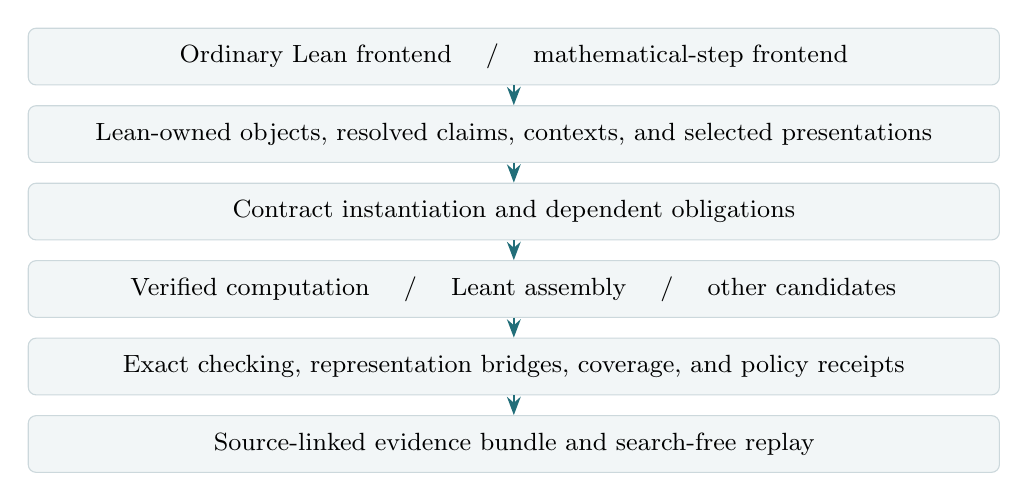
\begin{tikzpicture}[node distance=.25cm,
 box/.style={draw=linegray,fill=pale,rounded corners=1mm,text width=12.1cm,
 align=center,minimum height=.72cm,font=\small},>={Stealth}]
\node[box] (a) {Ordinary Lean frontend \quad / \quad mathematical-step frontend};
\node[box,below=of a] (b) {Lean-owned objects, resolved claims, contexts, and selected presentations};
\node[box,below=of b] (c) {Contract instantiation and dependent obligations};
\node[box,below=of c] (d) {Verified computation \quad / \quad Leant assembly \quad / \quad other candidates};
\node[box,below=of d] (e) {Exact checking, representation bridges, coverage, and policy receipts};
\node[box,below=of e] (f) {Source-linked evidence bundle and search-free replay};
\foreach \x/\y in {a/b,b/c,c/d,d/e,e/f} \draw[->,thick,accent] (\x)--(\y);
\end{tikzpicture}
\end{center}
This is a proposed architecture, not a diagram of implemented modules.

The initial components are a Lean-native context and expression service, a
contract registry, a presentation registry, a verified polynomial library or
adapter, a bounded dispatcher, and a publication checker. The Haskell synthesis
engine remains behind the adapter. Rewriting Leant in Lean is not required to
establish the semantics of the boundary.

\subsection{One modest relative guarantee}
Suppose every accepted node is checked at its exact proposition in its recorded
telescope; every computational bridge is proved; shared substitutions are
compatible; and the final term is checked against the approved target under the
axiom policy. Then composing the checked terms gives a proof of that target.
This follows from dependent application and substitution in the host logic.

That is the extent of the paper-level logical guarantee. It does not establish
that a compiler implementing this design is correct, that the chosen target is
what a human intended, that a renderer is faithful, that methods are explanatory,
or that reconstruction will finish. Repeating the substitution argument at length
would not retire those risks. The acceptance gates below target them directly.

\subsection{Milestones that can fail informatively}
\begin{longtable}{@{}P{.12\textwidth}P{.42\textwidth}P{.38\textwidth}@{}}
\toprule
Stage & Deliverable & Acceptance gate\\
\midrule
\endhead
0 & Pin a compiled source sample and its exact statements. Instrument existing
Lean, without introducing new syntax. & Record actual goals, outcomes, and
latencies. Separate observed source counts from reconstructed proof work.\\
1 & One polynomial calculation plus a guarded real-expression bridge, with
source-linked evidence and replay. & Reject cancellation at $x=1$, altered
reification, an unproved guard, and forged native output. Replay with discovery
disabled.\\
2 & Finite reindexing and local differentiation through ordinary theorem
interfaces, available in both frontends. & Prove positive cases; reject a
missing endpoint and point-only equality. Preserve the source's algebraic and
locality assumptions.\\
3 & A formal-series definition template and finite-jet implementation, with
rational scalar transport. & Support arbitrary specified Abel solutions; handle
the constant coefficient; reject finite-jet-to-full-equality promotion.\\
4 & Leant adapter, exact displayed-edit replay, worker cancellation, and
transactional shared constraints. & Distinguish all outcome strengths, reject
stale origins, and preserve accepted object choices.\\
5 & Exact algebraic-root and validated-numeric packages as independent
extensions. & Check branch-sensitive denesting, root identity across refinement,
and exact residual-to-enclosure transport.\\
6 & A reading, authoring, and maintenance study on held-out mathematics. &
Report useful and failed tasks, total costs, and syntax's incremental value;
retain a library-only or view-only outcome if supported.\\
\bottomrule
\end{longtable}

Stages can have parallel engineering work, but no stage should be declared
complete merely because it has an attractive source example. Stage~1 must leave
a replayable checked artifact before the project grows the grammar or recruits
a large set of domain methods. Basic isolation is required as soon as untrusted
generated metaprograms are executed; hardening is not postponed solely because
the interface is a research prototype.

\subsection{Performance is part of the design, not a later optimization}
Avoid re-elaborating a long telescope from text for every tiny obligation. Keep
resolved terms in the Lean worker and share immutable contexts. The dispatcher
uses a cheap applicability check before expensive search, while the real
logical applicability remains the instantiated theorem and its checked premises.
Cache proved side conditions by exact scoped identity, not by their printed form.

The total budget includes candidate enumeration and verification; accepted-result
quotas alone do not bound a stream with many failed candidates. Reflection on
large certificates needs its own cost measurements. The system should report
whether time was spent in elaboration, discovery, normalization, checking, or
rendering. A language that saves ten visible lines but repeatedly rebuilds a
large expression can be a regression.

\subsection{What not to implement first}
Do not start with an unrestricted prose parser, a universal CAS type, general
symbolic integration, arbitrary analytic continuation, automatic selection among
all available representation routes, or learned methods installed without checked
contracts. These are possible later research programs, not shortcuts around the
small exact boundary. Also do not spend the first iteration building a large toy
checker in a different logic: the decisive experiment must operate on actual
Lean mathematical statements.

\section{Evaluation that separates the language from its infrastructure}\label{sec:evaluation}
\subsection{Use nested baselines, then targeted ablations}
A convincing comparison should distinguish five configurations:

\begin{tabularx}{\textwidth}{@{}P{.12\textwidth}Y@{}}
\toprule
Arm & Available facilities\\
\midrule
$L_0$ & Existing idiomatic Lean source.\\
$L_1$ & Refactored Lean with the same mathematical lemmas and annotated method
interfaces used by the proposal.\\
$L_2$ & $L_1$ plus obligation records, source-linked evidence, semantic notices,
and an argument rendering.\\
$L_3$ & $L_2$ plus definition templates, presentations, and verified computational
services, all callable from ordinary Lean.\\
$L_4$ & The mathematical-step frontend over exactly the same facilities as $L_3$.\\
\bottomrule
\end{tabularx}


The difference $L_4-L_3$ tests the new input form. The difference $L_3-L_2$
tests the integrated computational and representation layer. Targeted ablations
within compatible task families should separate definition-interface improvements
from computational improvements. A completely crossed experiment is not always
meaningful because some operations depend on their presentation package; the
experiment must report those dependencies rather than pretend all factors are
independent.

For each comparison, fix the mathematical argument where possible. The
alternative double-counting proof in the syntheses, for example, is an argument
improvement that both frontends should receive \cite{synthesis,blueprints}.
A language should not receive credit for a better proof hidden in its helper
library while the Lean baseline is forced to retain the worse one.

\subsection{Measure actual author and reader work}
Record authoring time to an accepted artifact, editing actions, failed attempts,
needed hints, and the mathematical choices the system could not infer. For
readers, ask for the proof's central idea, the role of a specific hypothesis,
the domain of a calculated identity, and the effect of a deliberate mutation.
Repair tasks should change an endpoint, a coefficient structure, a definition,
a local instance, a root specification, or a library declaration.

System measurements include median and tail latency, total candidate-checking
work, replay time, peak memory, certificate size, cancellation latency, and
cache invalidation. Exact target preservation and negative-case behavior are
hard requirements. Source length is a descriptive outcome, not a proxy for
comprehension, generality, or total work.

For a reusable package with engineering cost $E$, authoring costs $A_i$, and
repair costs $R_i$, report
\[
 C(N)=E+\sum_{i=1}^{N}(A_i+R_i)
\]
as well as the individual terms. Amortization should use actual held-out reuse,
not hypothetical thousands of future proofs. A special-purpose theorem that
encodes the benchmark answer is not a free language primitive.

\subsection{A held-out design suited to these repositories}
Use the three inspected ProveIt modules as development material, not the final
test set. Hold out modules before harvesting their individual obligations so that
near-identical subgoals from one proof do not fall into both development and
evaluation. Include at least one unfamiliar family and an already-short Lean
control. Preserve the exact environment before the target theorem and exclude
the target, aliases of it, downstream consequences, and answer-bearing caches
from provider retrieval.

These exclusions prevent trivial environment leakage. They do not establish that
a pretrained model has never encountered the mathematics, so the evaluation must
not make that stronger claim. Inspect highly specialized helper lemmas for
answer leakage and report the allowed dependency closure.

Counterbalance frontend order and record Lean and mathematical experience.
Reading studies can compare generated and hand-authored argument views without
requiring every reader to learn a new language. Pilot measurements should set
practical acceptance thresholds; the present proposal does not invent a
percentage compression or speedup target.

\subsection{Decisions the results should be allowed to change}
If the polynomial and presentation packages help but the syntax does not, ship
the packages. If readers benefit from the argument view while authors prefer
Lean, ship the view. If a method wrapper costs more to maintain than the
underlying Lean proof, keep it out of the default profile. If Leant adds little
on single-lemma applications but helps on compositions, dispatch it selectively.

This is not a retreat from the design. The architectural thesis is that exact
mathematical interfaces and computational evidence should be shared. The input
surface is an empirical choice on top of that thesis.

\section{Research directions and limits}\label{sec:limits}
\subsection{The most promising extension: computation whose scope is visible}
Once exact polynomial and jet interfaces work, the same pattern can support
certified generating-function manipulation, recurrence solving in stated
fragments, root isolation, matrix certificates, and validated asymptotic bounds.
Each extension needs its own meaning relation and completeness claims. For
example, a formal asymptotic manipulation is not an error bound until its
remainder and domain have been proved.

A useful research problem is \emph{contract-directed presentation planning}:
given a fixed target relation and a bounded set of registered views, find a cheap
route with provable guards. Cost can include proof size, execution cost, and
reader-visible complexity. The planner is untrusted; the route checker is
simple. The hard open engineering issue is whether a useful route language stays
small as the library grows. The three-stage cast example and finite-jet precision
loss are initial stress tests, not evidence that the general problem is solved.

Another direction is learning reusable methods from accepted calculations.
A mined pattern should be generalized into an ordinary theorem or verified
algorithm, proved, versioned, and tested on held-out examples before becoming an
automatic method. Repetition in successful source code does not itself establish
the validity of the generalized rule.

\subsection{Concision has an irreducible mathematical component}
No interface can safely hide the choice of a useful invariant, an analytic
domination argument, a branch, or a representation when that choice carries the
substance of the proof. Better notation and better computation can make that
choice easier to express, but an automatic guess is still a guess until checked.
The goal is not a fixed maximum number of lines per theorem. It is to make each
visible line correspond to a meaningful mathematical commitment and to make
routine consequences cheap to reconstruct and inspect.

\subsection{What this article does and does not establish}
The mathematical derivations in the worked examples are supplied explicitly.
The source review identifies concrete interfaces and preserves their stated
generality. The supplementary Python script checks selected finite algebraic
calculations exactly with rational and integer arithmetic; it is neither a
formal proof nor a prototype of the proposed language. No new Lean source,
verified algorithm implementation, compiler correctness proof, whole-corpus
build, or usability experiment is delivered here.

The proposal is therefore falsifiable but not validated. Its most important
uncertainties are the cost of presentation infrastructure, the predictability
of reconstruction, and whether users benefit from the new source form. The
milestones and baselines are designed to distinguish those questions rather
than conceal them behind a polished example.

\section{Conclusion}
The first round's claim-centered Lean layer is the right foundation. The second
round should give it mathematical objects that are pleasant to compute with,
not merely more pleasant words for requesting proofs. \Facet{} proposes that
an object keep its identity while acquiring exact or observational presentations;
that every computation expose its relation, guards, and evidence; and that
verified algorithms, certificate search, and heuristic suggestions meet the same
precise checking boundary without being confused with one another.

This design addresses the user-visible reason a CAS can feel easier than a proof
assistant: the user can ask for a meaningful transformation and receive a usable
mathematical result. It rejects the corresponding danger: a result whose domain,
branch, coefficient structure, or logical strength changes silently. A practical
first outcome is a Lean library, a checked computational core, and a readable
argument view. A new language earns its place by making that shared workspace
better to author, read, and maintain.

\appendix
\clearpage
\section{A minimal implementation-facing interface}\label{app:interface}
The following is interface pseudocode. It is not a claim that these declarations
already exist in Lean or Leant. Logical fields become ordinary Lean types and
proofs; operational metadata remains separate.

\par\noindent\begin{minipage}{\linewidth}
\begin{lstlisting}
ExactPresentation A:
  Data       : Type
  valid      : Data -> Prop
  decode     : {d : Data // valid d} -> A

Presented (P : ExactPresentation A) (a : A):
  data       : P.Data
  validity   : P.valid data
  represents : P.decode (data, validity) = a

Observation A:
  Data       : Type
  relates    : Data -> A -> Prop
  -- No automatic equality reflection or unique decoding.

CalculationContract (input : A):
  Output     : Type
  relation   : Output -> Prop
  -- Domain and branch conditions are inside the exact proposition.

CertifiedResult (C : CalculationContract input):
  output     : C.Output
  evidence   : C.relation output

CheckedRoute:
  origin     : ResolvedContextAndInput
  edges      : InstantiatedBridgeTheorems
  guards     : OrderedDependentEvidence
  conclusion : ExactRelation
  proof      : ProofOfConclusion
\end{lstlisting}
\end{minipage}\par


A generic conditional result is a function over its guard telescope returning a
\code{CertifiedResult}. Operations with output types depending on input or guard
witnesses use the corresponding dependent version, not an erased uniform
\code{Output} container. A production schema must preserve those dependencies.

A deliberately small core syntax can be described as follows. \code{term} is a
host Lean expression; higher-level sketches in the article are proposed sugar
for these forms, not an implemented grammar.
\par\noindent\begin{minipage}{\linewidth}
\begin{lstlisting}
block      ::= step*
step       ::= claim id : term reason
             | calculate term relation term reason
             | obtain pattern from term
             | choose id : term satisfying term reason
             | within telescope { block }
             | cases term { branches }
             | induct term motive term { branches }
             | lean { host_tactic_block }
reason     ::= by method-id using references
             | by auto profile-id
relation   ::= equal | implies | equivalent
             | equal_on term | agrees_through term | enclosed_by
\end{lstlisting}
\end{minipage}\par


The semantic contract, not the keyword, determines the output type. In
particular, \code{agrees_through} must name its index convention and
\code{equal_on} its domain. A registered extension may add relation forms only
with a typed interpretation and checked composition rules. The initial
implementation should avoid heuristic relation-strength inference.

\section{Responses to the first synthesis's ten questions}\label{app:questions}
Identifiers S1--S10 follow the order in \emph{Mathematical Ideas, Checked Evidence}
\cite{synthesis}. Each answer is a proposed decision, not a reported experiment.

\begin{longtable}{@{}P{.07\textwidth}P{.39\textwidth}P{.46\textwidth}@{}}
\toprule
ID & Decision & Observation that should change or confirm it\\
\midrule
\endhead
S1 & Start with an ordinary theorem behind a stable interface; retain a typed
ledger for scope, guards, and policy. & Implement the same reindexing both with
and without the extra interface. Compare input effort and diagnostic precision,
not only successful proof length.\\
S2 & Named mathematical methods are constrained by their contract; \code{auto}
is explicitly open-ended. & Readers must distinguish a failed advertised map
from a valid alternative proof. If the distinction is confusing, revise the UI,
not the mathematical contract.\\
S3 & Only evidence-only changes and certified representation changes of the same
retained object are silent by default. & Mutate an induction motive, a root
branch, a local structure, and a hypothesis. All meaning-bearing changes must
produce reviewable edits.\\
S4 & Progress, root completion, exact displayed-edit replay, and policy acceptance
are independent receipt fields. & A tactic emitting invalid replacement text,
an admitted subproof, timeout, and undo must exercise different outcomes.\\
S5 & Share all infrastructure with Lean and charge its construction and repair
costs. & Held-out reuse determines whether a wrapper is broadly useful or merely
encodes a demonstration.\\
S6 & Pin selected routes; require explicit selection or a coherence theorem for
competing routes at the required observation. & The guarded natural-to-rational
route and a competing floor-based route must not change an accepted meaning.\\
S7 & Show domains, dependencies, conventions, structures, and relation strength,
not only a raw expression hash. & Ask readers to distinguish natural subtraction,
quantifier order, branch selection, and formal versus analytic series.\\
S8 & Keep evidence authoritative for its pinned environment and source useful
for explicit migration. & Rename a lemma, then change a definition. Measure
repair and whether a semantic change is disclosed.\\
S9 & Start definition authoring with a series-law template and finite presentations;
do not require a full new definition language. & Compare two representations
under the same specification and downstream tasks, through both frontends.\\
S10 & Expose mathematical choices and essential premises; collapse repeated checked
mechanics. & Measure missing-assumption localization, especially locality and
analytic premises, rather than preference for shorter pages.\\
\bottomrule
\end{longtable}

\section{Responses to the second synthesis's twelve questions}
Identifiers B1--B12 follow the order in \emph{Nine Blueprints} \cite{blueprints}.

\begin{longtable}{@{}P{.07\textwidth}P{.39\textwidth}P{.46\textwidth}@{}}
\toprule
ID & Decision & Observation that should change or confirm it\\
\midrule
\endhead
B1 & Build the document view first; keep the step input form optional. & Compare
lifted Lean, generated argument views, and hand-authored steps on the same
reading and repair tasks.\\
B2 & Treat routine as an empirical profile, not a global classification. & Measure
no-hint closure, closure with the author's hints, and failures separately under
fixed budgets.\\
B3 & Use small local-equality and derivative interfaces plus a composite theorem
for repeated patterns. & Compare applicability and failure explanations against
raw filter wrappers on held-out local-analysis goals.\\
B4 & Bind roles to project-owned typed interfaces, implemented by explicit theorem
applications; do not infer roles just from \code{Prop}. & Upstream renames should
break a small adapter, not silently change role meaning. Charge the adapter
maintenance cost.\\
B5 & Record dismissals per resolved construction; project defaults may suppress
categories but remain visible in the manifest. & Measure false alarms and
whether relevant meaning changes invalidate old dismissals.\\
B6 & Store source and evidence, with environment-specific authority. An upgrade
creates a new artifact rather than choosing a winner between incompatible ones.
& Compare replay cost and explicit repair after a rename and after a semantic
library change.\\
B7 & Keep provider reports separate from checker receipts; abstraction logs and
dependency records are different. & Adapt Leant, a tactic producer, and a model;
test non-derivability versus mathematical negation explicitly.\\
B8 & Dispatch Leant where measured gains justify it, especially structural
composition, rather than mandating it for every goal. & Separate single-lemma
applications from multi-premise compositions and compare with existing search.\\
B9 & Publish the selected data object and its exact specification; retain
alternatives in optional exploration history. & Test whether alternatives improve
understanding or merely distract from the accepted branch or behavior.\\
B10 & Begin with definition notices and a small number of proved templates. & Trace
recurring representation bridges to their originating definitions; compare the
cost of fixing the interface against repeated proof-level repair.\\
B11 & Namespaced contracts have explicit owners; conflicting operational profiles
require lexical or explicit selection, never import-order luck. & Have a second
author use two independently maintained packages and repair a policy upgrade.\\
B12 & Declare a Lean-library or document-view outcome successful in advance. &
Adopt the new input language only if it adds value over the equally equipped
Lean frontend, not because the project was initially called a language project.\\
\bottomrule
\end{longtable}

\section{Acceptance tests for the semantic boundary}\label{app:tests}
These are tests to implement with the language. They were not run as Lean tests
for this article. Each negative neighbor has a corresponding useful positive
operation; a system that simply refuses every case would not pass.

\begin{longtable}{@{}P{.06\textwidth}P{.44\textwidth}P{.42\textwidth}@{}}
\toprule
ID & Positive case and negative neighbor & Required result on the negative case\\
\midrule
\endhead
T1 & Cancel $(x-1)$ under $x\ne1$; then set $x=1$ in the total-function statement.
& Reject the unconditional equality or return the correct domain-restricted
relation; do not reinterpret it in $\Q(X)$.\\
T2 & Normalize polynomials over $\mathbf F_2$; then infer $X^2-X=0$ from its zero
evaluation function. & Refuse equality reflection without a valid injectivity
hypothesis.\\
T3 & Transport an integer equality to a quotient ring; then reflect equality
back along $\Z\to\mathbf F_2$. & Require reflection evidence; a ring homomorphism
alone is insufficient.\\
T4 & Reindex an inclusive finite interval; omit the final index. & Identify failed
coverage at the endpoint and preserve the original advertised method.\\
T5 & Differentiate a neighborhood identity; replace it by equality at one point.
& Request eventual equality, not unrelated stronger smoothness.\\
T6 & Invert a known unit; try to invert $2$ in $\Z$ using only $2\ne0$. & Leave a
unit obligation and retain the integer coefficient structure.\\
T7 & Compare jets through $N$; compare $0$ and $X^{N+1}$ as full series. & Report
only finite coefficient agreement, not full equality.\\
T8 & Differentiate a jet through $N+1$ to order $N$; supply only order $N$. &
Lower the output precision or request the missing coefficient.\\
T9 & Accept $\sqrt3-\sqrt2$ in the denesting example; propose its negative. &
Reject the principal-root specification despite identical squares.\\
T10 & Construct one root with isolation; label that result as all roots. & Require
coverage evidence for the all-roots contract.\\
T11 & Check a theorem with true auxiliary claims; insert a false unused claim. &
Reject the formal document even if the final theorem still has another proof.\\
T12 & Report complete intuitionistic search failure for excluded middle; call it
its mathematical negation. & Keep non-derivability separate; accept a negation
only with its exact proof.\\
T13 & Check a verified algorithm's computed output; alter one returned coefficient.
& Reject the output despite a genuine general correctness theorem for the
algorithm.\\
T14 & Accept a reply at its original scope; reuse it after undo or in a sibling
case with the same printed hypothesis names. & Reject the stale origin or
invalid context transport.\\
T15 & Use a formal identity coefficientwise; treat it as an analytic function
identity without a realization theorem. & Name the missing analytic bridge and
its premises.\\
T16 & Keep a conditional result under its guard telescope; use it unconditionally
or interchange dependent witness quantifiers. & Reject the scope or dependency
change, even when the printed expressions look similar.\\
\bottomrule
\end{longtable}

\clearpage
\section{Sources, provenance, and reproducibility}\label{app:sources}
The review is pinned to the following repository identities. These identify the
source evidence of this article, not a tested installation of the proposed
system.

\begin{description}[style=nextline]
\item[Brainstorm]
\code{494be9d5ab41a5ae219fc6f800e6aee3c93bce39}. Both requested synthesis texts
were reviewed, including their next-iteration questions and mutual corrections.
The nine individual reports are discussed through those syntheses; this article
does not claim to have independently re-reviewed all nine.
\item[ProveIt]
\code{7c4e3f109405b9805b35d27ae96bf09c7ee5f3d5}. Inspected
\code{BinomialInversion.lean}, \code{AutonomousIteratedDeriv.lean}, and
\code{AbelPolynomialSeries.lean} under
\path{Analysis/FabiusFunction/Lean/FabiusFunction/}.
This is the common comparison revision used by the syntheses, not a claim about
the latest ProveIt commit.
\item[Leant]
\code{3a40904be8a410d832d9ab6900b3d3e7b425eccb}. Inspected
\path{src/Leant/Synth/Verification.hs} lines 1--225,
\path{src/Leant/Synth/Engine.hs} lines 1--165, and
\path{src/Main.hs} lines 4700--4995, especially the suggestion and callback
boundaries. No Leant executable or regression suite was run.
\end{description}

The companion \code{source-manifest.json} records full paths, revisions, and
available blob identities. It distinguishes public committed sources from the
working-tree observations attributed to the earlier reports. Online reference
manuals are cited as consulted in September 2026, not treated as a pinned Lean
or Mathlib installation.

The article source is self-contained apart from standard LaTeX packages and
builds with \code{latexmk -pdf facet.tex}. The archive also contains a small
exact-arithmetic sanity-check script and its output. Those checks cover finite
binomial kernels, displayed derivative polynomials, finite Abel coefficients,
and several counterexample calculations. They provide reproducible consistency
checks for the exposition, not a formal verification of the proposed algorithms
or language. The PDF was compiled and visually inspected after rendering.

\clearpage
\begin{thebibliography}{99}
\small\raggedright
\addcontentsline{toc}{section}{References}

\bibitem{synthesis} Codex.
\emph{Mathematical Ideas, Checked Evidence: A Unified Evaluation of Nine
Proof-Language Proposals}. Brainstorm, 5 September 2026.
\path{docs/synthesis/unified-report.tex}.
\src{https://github.com/VladimirReshetnikov/Brainstorm/blob/494be9d5ab41a5ae219fc6f800e6aee3c93bce39/docs/synthesis/unified-report.tex}{Pinned report at revision 494be9d5}.

\bibitem{blueprints} Claude.
\emph{Nine Blueprints for a Mathematician's Proof Language over Lean}.
Brainstorm, 5 September 2026, revised synthesis.
\path{docs/unified_report/unified_report.tex}.
\src{https://github.com/VladimirReshetnikov/Brainstorm/blob/494be9d5ab41a5ae219fc6f800e6aee3c93bce39/docs/unified_report/unified_report.tex}{Pinned report at revision 494be9d5}.

\bibitem{p-binomial} Vladimir Reshetnikov and contributors.
\emph{ProveIt: BinomialInversion.lean}. Revision \code{7c4e3f10},
\path{Analysis/FabiusFunction/Lean/FabiusFunction/BinomialInversion.lean}.
\src{https://github.com/VladimirReshetnikov/ProveIt/blob/7c4e3f109405b9805b35d27ae96bf09c7ee5f3d5/Analysis/FabiusFunction/Lean/FabiusFunction/BinomialInversion.lean}{Pinned source}.

\bibitem{p-ode} Vladimir Reshetnikov and contributors.
\emph{ProveIt: AutonomousIteratedDeriv.lean}. Same revision and directory.
\src{https://github.com/VladimirReshetnikov/ProveIt/blob/7c4e3f109405b9805b35d27ae96bf09c7ee5f3d5/Analysis/FabiusFunction/Lean/FabiusFunction/AutonomousIteratedDeriv.lean}{Pinned source}, especially
\code{AutonomousODE.iteratedDeriv_eq_comp}.

\bibitem{p-abel} Vladimir Reshetnikov and contributors.
\emph{ProveIt: AbelPolynomialSeries.lean}. Same revision and directory.
\src{https://github.com/VladimirReshetnikov/ProveIt/blob/7c4e3f109405b9805b35d27ae96bf09c7ee5f3d5/Analysis/FabiusFunction/Lean/FabiusFunction/AbelPolynomialSeries.lean}{Pinned source}, especially
\code{coeff_exp_subst_of_abel_eq}.

\bibitem{l-verification} Vladimir Reshetnikov and contributors.
\emph{Leant: Leant.Synth.Verification}. Revision \code{3a40904b},
\path{src/Leant/Synth/Verification.hs}.
\src{https://github.com/VladimirReshetnikov/Leant/blob/3a40904be8a410d832d9ab6900b3d3e7b425eccb/src/Leant/Synth/Verification.hs}{Pinned source}, lines 1--225.

\bibitem{l-engine} Vladimir Reshetnikov and contributors.
\emph{Leant: Leant.Synth.Engine}. Same revision,
\path{src/Leant/Synth/Engine.hs}.
\src{https://github.com/VladimirReshetnikov/Leant/blob/3a40904be8a410d832d9ab6900b3d3e7b425eccb/src/Leant/Synth/Engine.hs}{Pinned source}, lines 1--165.

\bibitem{l-main} Vladimir Reshetnikov and contributors.
\emph{Leant: Main}. Same revision, \path{src/Main.hs}.
\src{https://github.com/VladimirReshetnikov/Leant/blob/3a40904be8a410d832d9ab6900b3d3e7b425eccb/src/Main.hs}{Pinned source}, lines 4700--4995.

\bibitem{lean-validation} Lean development team.
\emph{Validating a Lean Proof}. Lean Language Reference, consulted September 2026.
\url{https://lean-lang.org/doc/reference/latest/ValidatingProofs/}.

\bibitem{ring} Mathlib contributors.
\emph{Mathlib.Tactic.Ring.Basic}. API documentation, consulted September 2026.
\url{https://leanprover-community.github.io/mathlib4_docs/Mathlib/Tactic/Ring/Basic.html}.

\bibitem{harrison} John Harrison and Laurent Th\'ery.
A sceptic's approach to combining HOL and Maple.
\emph{Journal of Automated Reasoning} 21 (1998), 279--294.
\url{https://www.cl.cam.ac.uk/~jrh13/papers/cas.html}.

\bibitem{holcas} Cezary Kaliszyk and Freek Wiedijk.
\emph{Certified Computer Algebra on top of an Interactive Theorem Prover}.
Author-hosted paper.
\url{https://www.cs.ru.nl/~freek/pubs/holcas.pdf}.

\bibitem{coqeal} Maxime D\'en\`es, Anders M\"ortberg, and Vincent Siles.
\emph{A Refinement-Based Approach to Computational Algebra in Coq}.
Author-hosted paper, 2012.
\url{https://staff.math.su.se/anders.mortberg/papers/coqeal.pdf}.

\bibitem{afp} Ren\'e Thiemann, Akihisa Yamada, and Sebastiaan J. C. Joosten,
with contributions from Manuel Eberl.
\emph{Algebraic Numbers in Isabelle/HOL}. Archive of Formal Proofs,
entry dated 22 December 2015; current entry consulted September 2026.
\url{https://isa-afp.org/entries/Algebraic_Numbers.html}.

\bibitem{interval} Guillaume Melquiond and contributors.
\emph{Interval Package for Rocq}. Project documentation, consulted September 2026.
\url{https://coqinterval.gitlabpages.inria.fr/}.

\end{thebibliography}
\end{document}
